\chapter{Propriétés d'un désordre de type speckle}
\label{ch:Speckle}
%\begin{tikzpicture}[remember picture, overlay]
%\node[anchor=north east,inner sep=0pt] at (current page.north east) {
\includegraphics[scale=1]{Fig/Speckle/g825.png}};
%\end{tikzpicture}

Le chapitre \ref{ch:BEC_manip} nous a renseigné quant aux propriétés de notre onde de matière ainsi que sa production. En particulier, on a vu qu'il était possible d'appliquer des potentiels externes conservatifs aux atomes par le biais du potentiel dipolaire. Ce potentiel étant proportionnel à l'intensité lumineuse $I$, on peut alors appliquer un désordre à nos atomes, pourvu que l'on soit capable de créer un désordre optique. En effet, une originalité de notre expérience est "d'inverser" les rôles habituels de la matière et de la lumière.

Ainsi, dans ce chapitre, nous allons nous attacher à décrire le second élément clé de la localisation d'Anderson: le désordre. Nous montrerons que la génération d'un tel désordre est aisée: la diffraction d'un faisceau laser au travers d'une lame de verre rugueuse produit un motif d'intensité lumineuse aléatoire et à fort contraste, appelé champs de tavelures optiques, ou encore \emph{Speckle} (anglicisme communément admis). Citons deux énormes avantages d'un tel désordre: on en connaît toutes les propriétés, régies par la diffraction, et on contrôle ce désordre. 

La première partie se concentrera sur la génération d'un champ de speckle, en particulier sur le diffuseur qui donne au speckle toutes ses propriétés. Dans un second temps, nous décrirons les propriétés spatiales d'un speckle, en particulier la taille des grains de lumière dans les directions transverses et longitudinale. Dans une troisième partie nous parlerons du potentiel ressenti par les atomes ainsi que des possibilités offertes par la structure multi-niveaux du \isotope[87]{Rb} et l'excellent contrôle du désordre dont nous disposons, puis dans une ultime partie nous étudierons une approche à deux longueurs d'onde pour dépasser les limitations d'un speckle monochromatique pour l'étude de la transition d'Anderson à énergie résolue. 

\section{Génération d'un champ de speckle}
%\section{Propriétés statistiques d'un champ de speckle}
C'est avec le développement des premiers lasers qu'a été observée la structure granulaire de la lumière réfléchie par certaines surfaces rugueuses. Rapidement, il a été compris que ce motif provenait de la diffraction aléatoire et cohérente par une surface rugueuse. 
Cette surface rugueuse peut-être considérée comme un ensemble d'émetteurs cohérents de déphasages aléatoires, et le profil d'intensité obtenu est le résultat de l'interférence multiple de l'ensemble de la surface. Un profil typique est montré figure \ref{fig:speckle_pattern}. Celui-ci comporte un ensemble de grains lumineux séparés par des zones d'obscurité.
Souvent considéré néfaste dans le domaine de l'imagerie, le speckle est pour nous une formidable source de désordre optique. 

\begin{figure}
\centering
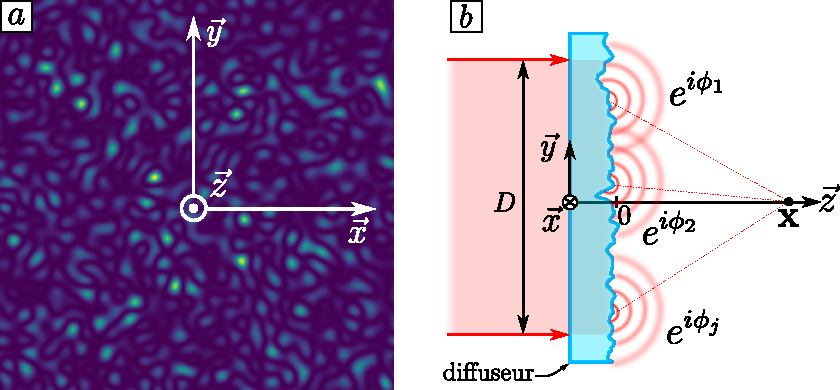
\includegraphics[scale=1]{Fig/Speckle/speckle_pattern.pdf}
\caption{\textbf{a:} Motif de speckle. Un tel motif est composé de grains lumineux entourés de zones d'ombre, où l'intensité est quasiment nulle. \textbf{b:} Génération d'une figure de speckle. La diffraction d'une onde cohérente par une surface rugueuse appelée diffuseur résulte en l'interférence multiple d'une grand nombre d'ondes à déphasage aléatoire. La phase de chacune de ces ondes est déterminée par l'épaisseur de verre traversée en chaque point.}
\label{fig:speckle_pattern}
\end{figure}



\subsection{Statistiques de l'intensité d'un speckle}
Modèle simpliste d'un grand nombre de diffuseurs qui émettent chacun une phase aléatoire. Le champ rayonné au point d'observation correspond à la somme de tous ces champs émis, ça fait une marche aléatoire dans le plan complexe. Dans ce cas, le théorème central limite donne pour les parties réelle et imaginaire de l'amplitude. Pour l'intensité, ça se traduit par une exponentielle décroissante.

Cette analyse repose sur 2 hypothèses: on a besoin d'un grand nombre d'émetteurs ($r_{\mathrm{diff}} \ll D$) et besoin d'une répartition homogène des phases ($\sigma_\phi \gg 2\pi$).


\begin{comment}
Marche aléatoire dans le plan complexe pour $\vec{E}$ car $\sigma_{\phi} \gg 2\pi$ ce qui valide l'approche de marche aléatoire (faire une figure de marche aléatoire avec beaucoup d'angles différents pour monter que $\left\langle t \right\rangle\approx 0$, et que sinon $\left\langle t \right\rangle\neq 0$.

Dans la partie d'avant, c'était au niveau du diffuseur. Maintenant on va s'attacher à décrire ce qu'il se passe après propagation. 
En première approximation, on peut supposer que le champ rayonné est la somme des $N$ champs émis par les diffuseurs avec des phases aléatoires:
\begin{equation}
E(\mathbf{x})=\sum_{j}^{N} E_0 e^{i \phi_j}
\end{equation}

\begin{figure}
\centering
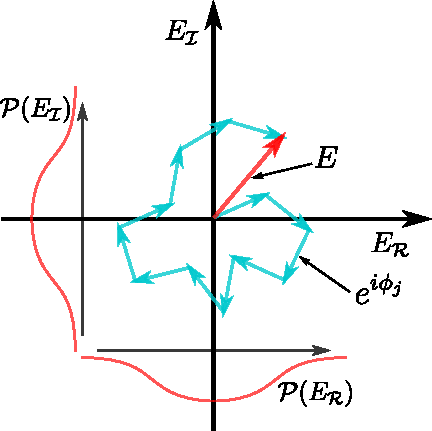
\includegraphics[scale=1]{Fig/Speckle/random_walk_speckle.pdf}
\label{fig:random_walk_speckle}
\caption{Marche aléatoire dans le plan complexe $E_{\mathcal{R}},E_{\mathcal{I}}$ dans le cas où $\sigma_{\phi} \gg 2\pi$}
\end{figure}
Théorème central limite car $r_{diff} \ll D$, $D$ étant la taille typique de l'éclairement incident.
\begin{equation}
\mathcal{P}(E_{\mathcal{R,I}})=\frac{1}{\sigma_E\sqrt{2\pi}} e^{-\frac{E_{\mathcal{R,I}}^2}{2 \sigma_E^2}}
\end{equation}
avec $E_{\mathcal{R}}$ et $E_{\mathcal{I}}$ les parties réelle et imaginaire du champ complexe $E$ respectivement. En faisant l'intégration angulaire, on trouve 
\begin{equation}
\mathcal{P}(I)=\frac{1}{2\sigma_E^2}e^{-\frac{I}{2\sigma_E^2}}
\end{equation}
Cette loi de probabilité permet alors d'obtenir l'intensité moyenne $\overline{I}=2\sigma_E^2$ et l'écart-type en intensité $\sigma_I=\overline{I}$. Le contraste d'une telle figure de speckle est alors de 1, ce qui se traduit par des pics très brillants entourés de régions sombres d'intensité quasinulle.
\end{comment}






\subsection{Propriétés du diffuseur}
\label{sec:propriete_diffuseur}
Lien des hypothèses précédentes avec les propriétés du diffuseur.
expression de la phase, de la transmittance moyenne, et de la correlation du diffuseur. lien avec $\sigma_\phi$ et $r_{\mathrm{diff}}$ pour connecter avec la partie précédente. Speckle pleinement développé.

\begin{comment}
Avant de nous intéresser aux propriétés du désordre à proprement parler, commençons par nous concentrer sur celles de l'élément générant le speckle: le diffuseur. Il s'agit d'une lame de verre dépolie, d'épaisseur locale $e(\mathbf{x}_0)$ aléatoire. On supposera que cette lame a été dépolie de manière homogène, ainsi, la statistique de l'épaisseur ne dépend pas de la position considérée sur la surface du diffuseur. On assimilera donc la distribution de l'épaisseur à un processus stationnaire. 

La phase localement accumulée par le faisceau laser incident lors de la traversée du diffuseur étant proportionnelle à l'épaisseur traversée, cette phase $\phi(\mathbf{x}_0)$ est elle aussi une variable aléatoire donnée par:
\begin{equation}
\phi(\mathbf{x}_0)=2\pi (n-1) \frac{e(\mathbf{x}_0)}{\lambda}
\end{equation}
avec $n$ l'indice du verre et $\lambda\approx \SI{780}{\nano\metre}$ la longueur d'onde de l'onde laser.
L'effet de cette phase aléatoire locale se traduit en terme d'amplitude via la transmittance du diffuseur. De même que l'épaisseur et la phase, il s'agit d'une grandeur locale définie par:
\begin{equation}
t_{\mathrm{diff}}(\mathbf{x}_0)=e^{i\phi(\mathbf{x}_0)}
\end{equation}

\begin{equation}
\overline{t_{\mathrm{diff}}} = \overline{e^{i\phi}} = \int{\mathrm{d}\phi \: e^{i\phi} \mathcal{P}(\phi)} \quad\text{avec}\quad \mathcal{P}(\phi)=\frac{1}{\sigma_{\phi} \sqrt{2\pi}} e^{-\frac{(\phi-\overline{\phi})^2}{2\sigma_{\phi}^2}}
\end{equation}
En considérant que $\phi$ est une variable aléatoire gaussienne, ça donne
\begin{equation}
\overline{t_{\mathrm{diff}}}=e^{-\frac{\sigma_{\phi}^2}{2}}
\end{equation}
et en choisissant correctement l'origine temporelle telle que $\overline{\phi}=0$.

On peut aussi écrire $t_{\mathrm{diff}}$ sous la forme
\begin{equation}
t_{\mathrm{diff}}=\overline{t_{\mathrm{diff}}}+\delta t_{\mathrm{diff}}
\end{equation}
ce qui se traduit en terme de champ
\begin{equation}
E=\overline{E}+E_{speckle}
\end{equation}
La conséquence est alors immédiate: si $\sigma_{\phi} \gg 2\pi$ ou de manière équivalente $\sigma_e \gg \lambda$, alors $\overline{t_{\mathrm{diff}}} =0$ et donc le champ rayonné ne sera composé que du champ de speckle: on parle alors de speckle entièrement développé. La valeur déterministe $\overline{E}$ liée à $\overline{t_{\mathrm{diff}}}$ est supprimée. C'est ce que l'on considèrera dans la suite.

\begin{figure}
\centering
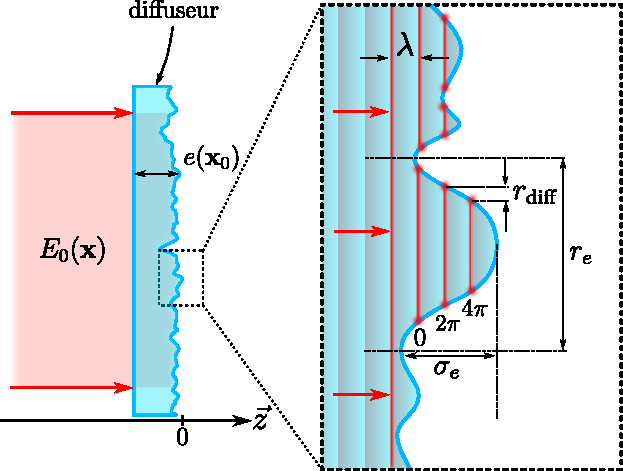
\includegraphics[scale=1]{Fig/Speckle/diffus_prop.pdf}
\label{fig:diffus_prop}
\caption{Caractéristiques du diffuseur. L'épaisseur aléatoire est caractérisée par une hauteur typique $\sigma_e$ et une granularité de taille $r_e$. Pour $\sigma_e \gg \lambda$, on a plusieurs oscillations de l'onde incidente dans le même grain, et donc $t_{\mathrm{diff}}$ qui est une fonction $2\pi-$périodique, voit sa corrélation réduite.}
\end{figure}

Fonction de corrélation: on définit
\begin{equation}
C_{\mathrm{diff}}(\mathbf{x}_0,\mathbf{x}'_0)=\overline{t_{\mathrm{diff}}(\mathbf{x}_0)t^*_{\mathrm{diff}}(\mathbf{x}'_0)}=\overline{e^{i(\phi(\mathbf{x}_0)-\phi(\mathbf{x}'_0))}}
\end{equation}
Si l'on suppose que $\phi(\mathbf{x}_0)-\phi(\mathbf{x}'_0)$ est aussi une variable gaussienne, ça donne
\begin{equation}
C_{\mathrm{diff}}(\mathbf{x}_0,\mathbf{x}'_0)=e^{-\sigma_{\phi}^2 (1-\overline{\phi(\mathbf{x}_0)\phi(\mathbf{x}'_0)}/\sigma_{\phi}^2)}
\end{equation}
Corrélations de l'épaisseur du diffuseur:
\begin{equation}
\frac{\overline{\phi(\mathbf{x}_0)\phi(\mathbf{x}'_0)}}{\sigma_{\phi}^2}=\frac{\overline{e(\mathbf{x}_0)e(\mathbf{x}'_0)}}{\sigma_e^2} \approx 1-\frac{\left| \mathbf{x}_0-\mathbf{x}'_0 \right|^2}{2r_e^2}
\end{equation}
courbe en cloche assez générale valable pour $\left| \mathbf{x}_0 -\mathbf{x}'_0 \right| \ll r_e$.

Au final, ça donne une corrélation de la transmittance 
\begin{equation}
C_{\mathrm{diff}}(\mathbf{x}_0,\mathbf{x}'_0)\approx e^{-\frac{\left| \mathbf{x}_0 - \mathbf{x}'_0 \right| ^2}{2 r_{\mathrm{diff}}^2}}
\end{equation}
avec $r_{\mathrm{diff}} = r_e / \sigma_{\phi}$ la taille effective des grains du diffuseur. Cette taille diminuée s'explique par le fait que si $\sigma_{\phi} \gg 2\pi$, la phase ne sera pas homogène sur la totalité de la largeur d'un grain (de taille typique $r_e$), mais seulement sur une zone réduite. 

\end{comment}



\subsection{Implémentation expérimentale}
À présent, étudions la géométrie de notre dispositif de génération du speckle. Le faisceau est émis par un laser Toptica TA-Pro 2W accordable autour de 780nm (Raie $\mathrm{D}_2$ du ${}^{87}\text{Rb}$). Cette accordabilité nous offre la possibilité de réaliser un potentiel désaccordé vers le rouge et donc attractif ($\delta < 0$) ou bien désaccordé vers le bleu, et donc avoir un potentiel répulsif ($\delta > 0$). Historiquement, le laser auparavant utilisé pour générer le speckle était un laser Verdi à 532nm très désaccordé vers le bleu afin de s'affranchir de l'émission spontanée, nécessaire sur des très longs temps pour l'étude de la localisation d'Anderson. Étant donnée la proximité de la résonance avec ce nouveau système autour de 780nm, nous travaillons à bien plus basse puissance (typiquement quelques µW). Le mode du laser est filtré à l'aide d'une fibre optique, sa polarisation est fixée linéaire à l'aide de cubes séparateurs de polarisations, et l'ensemble est asservi en puissance (l'essentiel de la puissance du laser sert d'ailleurs à cette boucle d'asservissement). Les détails de ce montage peuvent être retrouvés dans la thèse de Vincent Denechaud. 

\begin{figure}
\centering
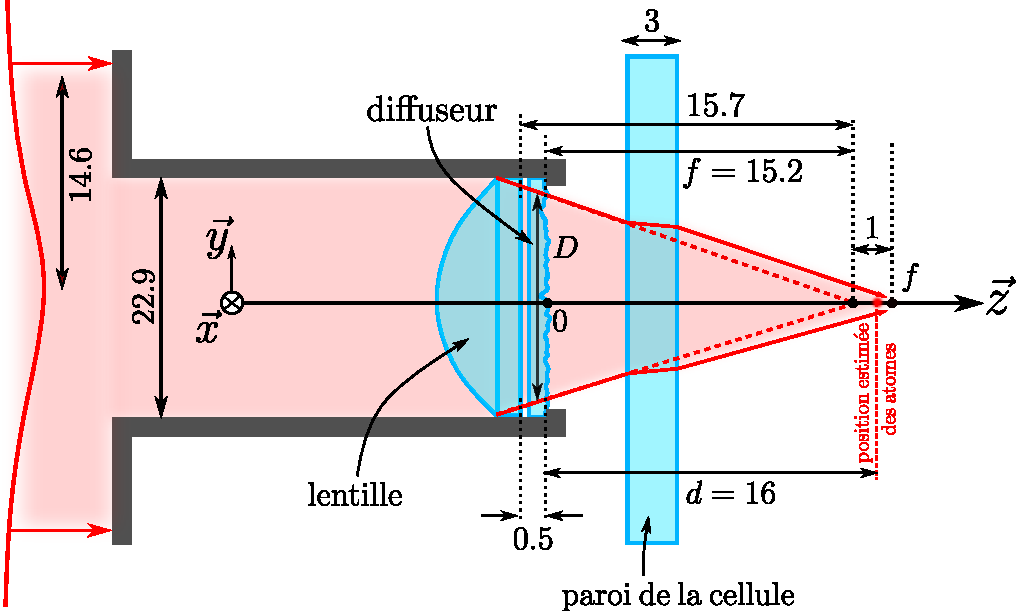
\includegraphics[scale=0.7]{Fig/Speckle/montage_diffuseur.pdf}
\caption{Géométrie du montage de génération du speckle. Un faisceau gaussien incident est tronqué dans un diaphragme qui supporte le diffuseur. Le plan de focalisation est déplacé d'environ 1mm à cause de la paroi de la cellule à vide.}
\label{fig:montage_diffuseur}
\end{figure}

La génération du speckle se fait donc selon le montage représenté figure \ref{fig:montage_diffuseur}. Un faisceau gaussien collimaté de taille 14.6mm est tronqué par un diaphragme de diamètre 22.9mm. Ce faisceau passe ensuite au travers d'une lentille asphérique (\textit{Thorlabs ACL2520-B}) de focale 16mm (et de frontale 15.7mm). Le diffuseur \textit{Newport FSD10-3} possède une épaisseur de 0.3mm (initialement 3mm avant d'être aminci par l'atelier d'optique de l'IOGS) et diffuse selon un angle $\theta_{\mathrm{diff}}\approx$ 5° (données constructeur). Le faisceau traverse ensuite la paroi de la cellule en vycor (d'indice optique $n=1.46$) d'épaisseur $e=3$mm. La présence de la paroi entraîne un déplacement du plan de focalisation de $\Delta d=e(1-1/n)\approx1$mm. En positionnant l'origine sur la surface du diffuseur, le plan de focalisation se trouve à $f=16.4$mm. La position des atomes est estimée quant à elle a $d=16\pm0.5$mm. L'incertitude liée à cette dernière position est primordiale: nous devons connaître les proriétés du speckle autour du plan de focalisation. 
{\Large TODO: Faire un calcul rapide d'ODG pour justifier la lentille: besoin de focaliser la lumière pour avoir un potentiel raisonable sur les atomes à puissance raisonnable.}



\section{Propriétés spatiales d'un champ de speckle}
Bien que les figures de speckle soient déterministes car régies par la diffraction, on peut considérer leurs réalisations comme étant aléatoires. Néanmoins, les propriétés spatiales d'un champ de speckle ne dépendent pas de la réalisation, mais seulement de la géométrie du problème. Dans cette section, nous allons nous attacher à décrire les grandeurs spatiales caractéristiques d'un speckle: son extension et la taille des grains, donnée par la fonction d'autocorrélation en intensité. Ces quantités on été mesurées expérimentalement sur un montage reproduisant exactement les conditions réelles de la cellule à vide, celle-ci empêchant de faire des mesures in-situ. La description de ces mesures et de leur traitement sont référencées dans la thèse de Jérémie Richard.

\subsection{Extension transverse du champ de speckle le long le l'axe optique}
Afin de connaître l'extension spatiale du champ de speckle, il nous faut dans un premier temps calculer l'amplitude rayonnée. Appliquons l'approximation paraxiale au principe de Huygens-Fresnel:
\begin{align}
E(x,y,d)&\propto \int{\mathrm{d}x_0 \mathrm{d}y_0 \: E_0(x_0,y_0) \: t_{\mathrm{diff}}(x_0,y_0) \: \exp{\left( -ik\frac{x_0^2+y_0^2}{2f} \right) } \: \exp{ \left( ik\frac{(x-x_0)^2+(y-y_0)^2}{2d} \right) }} \\
&\propto \int{\mathrm{d}x_0 \mathrm{d}y_0 \: E_0(x_0,y_0) \: t_{\mathrm{diff}}(x_0,y_0) \: \exp{\left( ik\frac{x_0^2+y_0^2}{2d_{\mathrm{eff}}} \right) } \: \exp{\left( -ik \frac{xx_0+yy_0}{d} \right) }}
\end{align}
avec $1/d_{\mathrm{eff}}=1/d-1/f$. Le profil d'intensité moyenne est donné par la fonction de corrélation en amplitude, évaluée aux deux mêmes points:
\begin{equation}
\overline{I}(x,y,d)=\overline{E(x,y,d)E^*(x,y,d)}
\end{equation}
On peut alors montrer que l'intensité moyenne est issue de la convolution de deux termes:
\begin{equation}
\overline{I}(x,y,d)\propto \left[ I_0(\frac{d_{\mathrm{eff}}}{d}x_0,\frac{d_{\mathrm{eff}}}{d}y_0) \ast \widetilde{C_{\mathrm{diff}}}(kx_0/d,ky_0/d) \right] (x,y)
\end{equation}
Explicitons la physique qui se trouve derrière cette formule. Pour cela, discutons des deux termes de la convolution. 

Le premier terme n'est autre que l'intensité incidente sur le diffuseur, redimensionnée par l'effet de la lentille. En effet, le changement d'échelle par $d/d_{\mathrm{eff}}=\left| d-f \right| /f$ montre qu'au cours de la propagation, la taille du faisceau en l'absence du diffuseur diminue jusqu'au plan de focalisation ($d=f$), puis augmente indéfiniment. Le caractère linéaire de cette loi d'échelle se comprend aisément dans le cadre de l'optique géométrique: le faisceau se focalise dans le plan $z=f$, où tous les rayons lumineux se croisent puis s'écartent. Il s'agit du terme prépondérant dans les régions éloignées du plan focal.

Le second terme traduit la diffraction des différents grains du diffuseur. Ces grains ont une taille typique $r_{\mathrm{diff}}$ et vont donc diffracter selon un angle $\theta_{\mathrm{diff}}=\lambda/r_{\mathrm{diff}}$. Cela va donc se traduire par une taille transverse $w_{\mathrm{diff}}=\theta_{\mathrm{diff}} d$, qui augmente linéraire avec la distance $d$. Il s'agit du terme prépondérant aux alentours du plan de Fourier. 

On a vu en section \ref{sec:propriete_diffuseur} que la fonction de corrélation $C_{\mathrm{diff}}$ est en bonne approximation une gaussienne. En supposant un éclairement incident gaussien (on néglige l'effet du diaphragme), 

\subsection{Longueur de corrélation transverse le long de l'axe optique}
Calcul de la corrélation transverse aux alentours du plan de Fourier, forme gaussienne bien reproduite car la pupille ne coupe que quelques \% de la lumière du faisceau laser gaussien incident: la TF d'une gaussienne faiblement tronquée est une gaussienne correcte.

\subsection{Corrélation longitudinale}
Calculs de la corrélation longitudinale. Formule de la thèse de Fred redémontrée en annexe. Application à un éclairement gaussien, et un éclairement homogène tronqué. Réalité entre les deux, donc la fonction de corrélaiton réelle est quelque part entre une lorentzienne et un sinus cardinal. C'est pas parfait partout, alors modélisation en tenant compte des effets non-paraxiaux pour vraiment reproduire la corrélation longitudinale. Calculs lourds numériquement et théoriquement, donc on met en place un modèle paraxial à ON effective. Avecun facteur de scaling sur la taille du faisceau incident et sur la pupille, on arrive à reproduire de manière convenable la corrélation longitudinale. Avantage: ça reste paraxial donc on peut en tirer des grandeurs. 

\section{Propriétés du potentiel de type speckle}
\subsection{Propriétés du potentiel}
Traduction de $P_I(I)$ pour le potentiel dipolaire $V$, Taille des grains de potentiel $\sigma$, potentiel moyen $V_{\mathrm{R}}$, possibilité de faire un potentiel attractif $\delta <0$ ou répulsif $\delta > 0$
\subsection{Possibilité d'un potentiel dépendant de l'état interne}
En choisissant un désaccord très petit vis à vis d'un état hyperfin, on peut réaliser un potentiel très grand sur cet état tandis qu'on peut le négliger pour le second état. Pour cela, il faut que le désaccord soit très petit devant la séparation hyperfine de ces états. Par contre, il faut garder un désaccord suffisamment grand pour continuer de pouvoir considérer ce champ comme un potentiel conservatif, sinon on va avoir des processus inélastiques. Exemple de mesure des fonctions spectrales, où le temps de vie à cause des processus inélastiques n'était que 100ms, très insuffisant pour l'étude de la localisation d'Anderson, qui nécessite des temps d'évolution dans le désordre de plusieurs secondes.

\section{Potentiel composé d'un speckle bichromatique}
\subsection{S'éloigner de résonance}
Grosse limitation de l'approche précédente utilisée pour les fonctions spectrales: implique qu'on est proche de résonance pour l'état $\left| F=2 \right\rangle$, donc taux d'absorption et d'émission spontanée important: grosse décohérence dans le désordre et donc impossible d'observer la localisation.
Donc on s'éloigne de résonance, donc le potentiel sur $\left| F=1 \right\rangle$ n'est plus négligeable, il faut le compenser: second speckle! 
\subsection{Étude de la similitude de deux speckles}
Physique avec les mains de la similitude entre 2 speckles de longueurs d'onde faiblement différentes. introduction de la finesse $\lambda / \delta\lambda$ ou de la longueur de cohérence $l_{coh}=\lambda^2/\delta\lambda$.
Décorrélation initiale et globale dûe à la propagation dans le diffuseur, puis décorrélation par la différence dans la taille des grains en s'éloignant de l'axe optique.